\documentclass{acm_proc_article-sp}

\usepackage{epstopdf}
\usepackage{auto-pst-pdf}
\usepackage{graphicx}
\usepackage[labelfont=bf]{caption}

\graphicspath{ {Includes/} }

\begin{document}

\title{A Farewell to Structural Rigidity}
\subtitle{Midterm Project Report}

\numberofauthors{3}
\author{
% 1st. author
\alignauthor Christopher Ross	
% 2nd. author
\alignauthor Jonathan Brant
% 3rd. author
\alignauthor Zak Roessler
}

\maketitle

\section{Introduction}
Image recognition and classification problems have long captured the interest of computer vision researchers \cite{shapiro2001computer, morris2004computer, sonka2008image}.  The ability to process and accurately identify visual input has a vast array of interesting applications across the field of AI and other scientific disciplines.  Unsurprisingly, however, such an undertaking has proven to be a rather ambitious, with one of the primary obstacles being that of scale \cite{DBLP:journals/corr/RussakovskyDSKSMHKKBBF14}.

Perhaps the most straightforward method of processing images is to consider each pixel as a separate input into an artificial neural network (ANN) classifier, with the image resolution defining the distinct number of pixels.  As image resolution increases, however, the number of classifier inputs will similarly grow exponentially, easily reaching inputs in the millions.  Considering each pixel separately quickly becomes an inefficient approach and necessitates a method for dimensionality reduction.

In order to tackle such large problems, this project proposes the use of an evolved autoencoder. Unlike traditional autoencoders wherein the hidden layers (i.e. compressed feature vectors) are specified apriori, the research presented herein uses HyperNEAT to evolve connective CPPNs which in turn produces autoencoders that are, for all practical purposes, scale invariant and whose hidden structure are decided in a more principled manner.


\section{Background}
The fundamentals of traditional autoencoders are introduced along with the relevant details of the HyperNEAT algorithm.

\subsection{Autoencoders}
Autoencoders are artificial neural networks that perform a non-linear form of principal components analysis (PCA) and attempt to extract the most salient features from the visible (input) layer \cite{bourland1988, baldi2012autoencoders}.  A simple autoencoder has a separate input/output pair for each "visible" feature of a domain as well as a fully connected hidden layer that learns the most salient features of the uncompressed features in the visible layer.  More generally, input is being encoded into a compressed representation and subsequently reconstructed.  Figure 1 depicts the structure and encode/decode phase of a simple autoencoder.

After the compressed feature vector outputs have been decoded into the full feature set, a reconstruction error is calculated and used to determine the representational efficiency/accuracy of the hidden layer.  The reconstruction error for each visible layer node is fed to a supervised training algorithm, most commonly backpropagation, which updates the weights of the autoencoder in a direction that minimizes reconstruction error \cite{stanfordimage}.

\begin{figure}[h]
\caption{An autoencoder with 6 visible units and 3 hidden units.  The input is encoded from Layer L1 to Layer L2, and decoded from Layer L2 to Layer L3 \cite{stanfordimage}.}
\centering
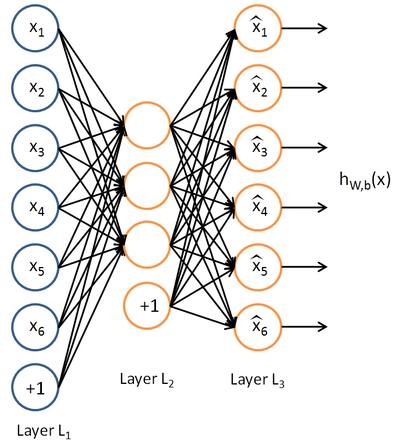
\includegraphics[scale=0.8]{ExampleAutoencoder}
\end{figure}

\subsection{NEAT}
In order to automatically determine the autoencoder’s hidden layer topology, techniques are borrowed from the field of neuroevolution.  One of the most successful and widely-used genetic algorithms for ANN evolution is the NeuroEvolution of Augmenting Topologies (NEAT).  Three primary components separated NEAT from algorithms that preceded it: growth from minimal structure, speciation, and perhaps most importantly, historical markings \cite{Stanley:2002:ENN:638553.638554}.

Prior to NEAT, many Topology and Weight Evolving Artificial Neural Networks (TWEANNs) began evolution in an already high-dimensional state, leading to slow computationally intensive evolution and often poor results.  NEAT addresses this issue by starting with minimal structure (no hidden nodes) and complexifying only when doing so positively impacts objective performance.  

A potential problem with starting minimally, however, is that such structure will be optimized over time, often out-performing new structural innovations that haven't yet had a chance to be fine-tuned.  NEAT's speciation component avoids premature penalization of new innovations by imposing explicit fitness sharing.  This allows an "adjusted fitness" to be calculated for each genome relative to other structurally similar genomes in its species, thus avoiding premature convergence and protecting new innovations.

Finally, at the core of NEAT are historical markings that uniquely identify each structural innovation.  Historical markings solve the topology matching problem, allowing crossover operations without expensive topological analysis.  Speciation also uses historical markings to determine the species in which to place each genome.

NEAT has been proven to be a highly successful algorithm for control and sequential decision tasks in relatively low-dimensional domains; however, as a direct encoding, the NEAT genotype contains a separate gene for each structural component.  For high-dimensional domains, this can quickly become unwieldy and difficult to optimize.  Moreover, as NEAT considers every input separately, it has no concept of geometric regularities making it a less than optimal choice for domains with a strong visual component.

\subsection{HyperNEAT}
Given the complexity of the domain under consideration and the strong geometric component, the Hypercube-based NeuroEvolution of Augmenting Topologies (HyperNEAT) is a natural choice of algorithms \cite{Stanley:2009:HEE:1516090.1516093}.

As an indirect encoding, HyperNEAT does not impose a one-to-one mapping between genes in the genotype and structural components (i.e. connections and neurons in the case of ANNs) in the phenotype. Instead, HyperNEAT evolves Compositional Pattern Producing Networks (CPPNs) that describe connectivity patterns as a composition of canonical functions \cite{Stanley:2007:CPP:1265496.1265517, Stanley:2009:HEE:1516090.1516093}.  The evolved CPPN queries every possible connection within a 2n-dimensional substrate and outputs the weight of the connection between those two points, effectively drawing an n-dimensional connectivity pattern which is then interpreted as an ANN and evaluated in the given domain.

\begin{figure}[h]
\caption{The "state-space sandiwch" substrate - ideal for visual mapping \cite{Stanley:2009:HEE:1516090.1516093}.}
\centering
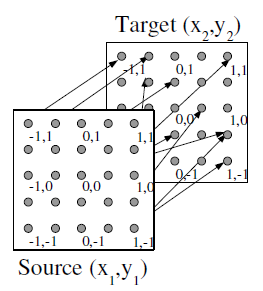
\includegraphics[scale=0.8]{StateSpaceSandwichSubstrate}
\end{figure}

The substrate configuration is hand-designed in order to accurately represent the geometry of the task-domain.  Among the many possible substrate configurations, one of the most widely used is the "state-space sandwich" substrate wherein a source sheet of neurons is fully connected to a target sheet, as shown in Figure 2.  A modified version of the state-space sandwich will be used to represent the visible and hidden layers of the desired autoencoder.  HyperNEAT’s ability to efficiently generate extremely large scale networks that exhibit virtually no loss of function while using a highly compressed representation that accounts for domain geometry makes it an ideal candidate for the image image processing tasks considered in this paper.

\section{Approach}
While autoencoders have been considered viable methods for data compression or dimensionality reduction since their introduction in 1988 \cite{bourland1988}, they have, to the author’s knowledge, always been statically constructed such that their hidden layer is fully specified apriori.  This paper seeks to evaluate the potential of leveraging HyperNEAT for the evolution of autoencoder hidden layer topology.  Results of such an approach will be analyzed both quantitatively (i.e. the efficacy of evolved topology toward reducing reconstruction error) and qualitatively (i.e. how closely does the reconstructed image resemble the original).

The substrate configuration should be chosen to match that of a typical autoencoder structure in order to capture the encode/decode concept.  This includes a two-dimensional sheet of neurons representing each pixel in the given image, a hidden layer sheet with fewer (typically half) neurons, which will in turn be connected to a sheet the same size as the input sheet.  The "hidden layer" sheet effectively represents the hidden layer of a traditional autoencoder.  This "stacked" state-space sandwich is depicted in figure 3.

\begin{figure}[h]
\caption{The "state-space sandwich" substrate used in the evolved autoencoder experiments.  The hidden layer may vary depending on the experiment configuration, but the general three-tiered structure will remain.}
\centering
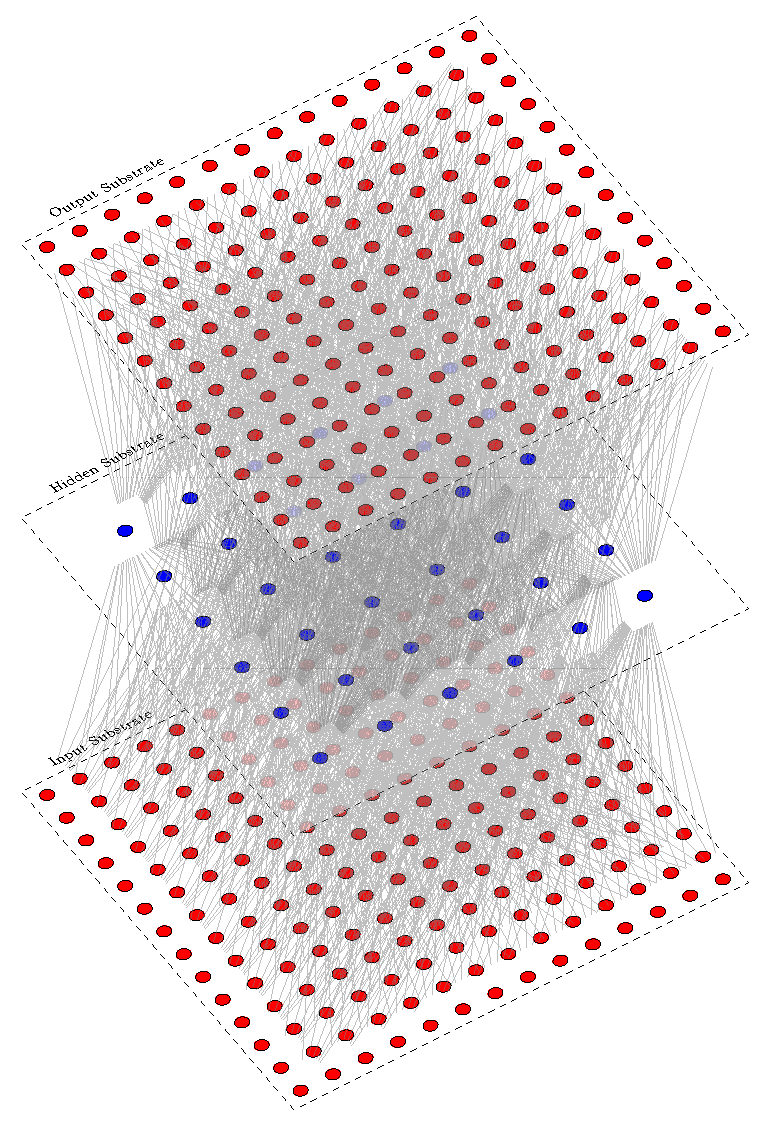
\includegraphics[scale=0.55]{SubstrateConfiguration/AutoencoderSubstrate}
\end{figure}

A HyperNEAT-evolved CPPN will query each possible connection between the input sheet and the hidden sheet as well as between the hidden sheet and the output sheet, outputting the weight for that connection (assuming the weight is of high enough magnitude for the connection to be expressed).  Evolution will begin with a minimally connected CPPN (no hidden nodes) with five input nodes and four output nodes.  The input nodes accept the Cartesian coordinates (x and y position values) for each line segment endpoint and a bias, while the output nodes express the connection weight for the line segment and the bias between the input sheet and the hidden sheet, as well as the same between the hidden sheet and the output sheet.  One such minimal CPPN is shown in figure 4.

The resulting connectivity pattern will be interpreted as an autoencoder and will be both trained and evaluated on samples from the Mixed National Institute of Standards and Technology (MNIST) handwritten digit dataset \cite{mnistdataset}, which is often used as a benchmark dataset for image classification problems.

\begin{figure}[h]
\caption{The minimal, starting-state (no hidden nodes) CPPN.  The inputs to the CPPN are the X and Y coordinates on the source substrate and the X and Y coordinates on the target substrate.  Depending on which layer the CPPN is querying, it will either output the weight of the connection between the input substrate and hidden substrate along with the weight of the bias connection between the same, or the weight of the connection between the hidden substrate and output substrate along with the weight of the bias connection between the same.}
\centering
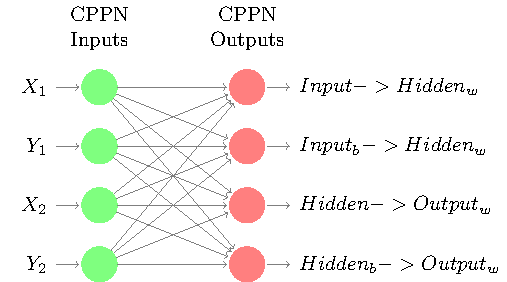
\includegraphics[scale=0.8]{MinimalCppn/MinimalCppn}
\end{figure}

The training process will use traditional backpropagation (though over arbitrary hidden layer topologies), modifying the autoencoder weights in order to reduce reconstruction error.  After backpropagation has been run for the specified number of iterations (which will vary based on the experiment configuration), the overall reconstruction error will be taken as the score of the CPPN that generated the autoencoder under evaluation.  Figure 3 describes the full process.

In this way, HyperNEAT is generating the autoencoder starting state and backpropagation is fine tuning it.  The hope is that HyperNEAT will generate a structure that is easily trained to a point of minimal reconstruction error.

%\balancecolumns

\section{Discussion of Current State}
The current state discussion includes the results observed thus far from initial experimentation, an analysis of those results (including alternate strategies in the event that experiment outcomes were poor), and final experiments that are planned to bring the project to a hopefully informative completion.

\subsection{NEAT Results}
During the initial stages of experimentation, standard NEAT was used to directly evolve autoencoders.  The result was slow evolution (due to the massive search space) and qualitatively poor image reconstruction.  Interestingly, while reconstruction error reached about 90\% accuracy form a quantitative standpoint, the qualitative result was a completely black image.  Intuitively, this was because most of the image was just empty, black space and the digit itself occupied a comparatively small number of pixels.

However, the deeper problems was that NEAT was unable to generate a viable autoencoder starting state due to its inability to account for task geometry.  It was primarily this realization that led to the incorporation of HyperNEAT.

\subsection{HyperNEAT Results}

Add HyperNEAT results here...

\subsection{Plan for Completion}

Add additional experiments that we want to run here...

\bibliographystyle{ieeetran}
\bibliography{MidtermReport}

\end{document}
